\documentclass[a4paper,fontset = windowsnew]{ctexbook}
\usepackage{xifthen}
\usepackage{calc}
\usepackage{graphicx}
\usepackage{tikz}
\usetikzlibrary{patterns}
%\usepackage{amsmath}
\usepackage[user=student]{cexam}

\begin{document}
\chapter{基本排版程序}


%\ExplSyntaxOn
%\parindent=0pt

\begin{choices}
  1.这是选择题的题干,如
  <<
  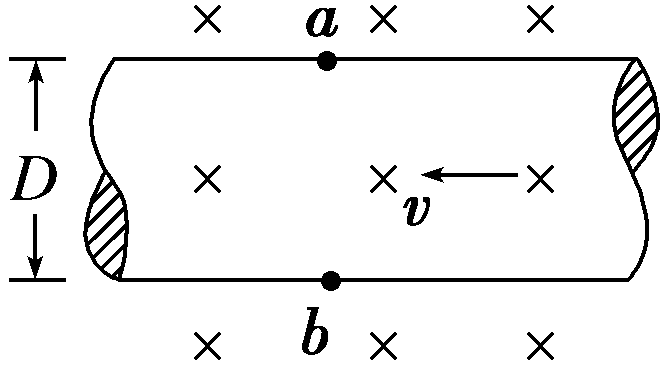
\includegraphics{1.png}
  >>
  所示是图片.其中有四个选项,分别是
  A.选项A这是长选项部分测试这是长选项部分测试这是长选项部分测试这是长选项部分测试这是长选项部分测试这是长选项部分测试这是长选项部分测试这是长选项部分测试这是长选项部分测试这是长选项部分测试这是长选项部分测试这是长选项部分测试这是长选项部分测试这是长选项部分测试
  B.选项B这是长选项部分测试这是长选项部分测试这是长选项部分测试这是长选项部分测试这是长选项部分测试这是长选项部分测试这是长选项部分测试这是长选项部分测试这是长选项部分测试这是长选项部分测试这是长选项部分测试这是长选项部分测试这是长选项部分测试这是长选项部分测试这是长选项部分测试这是长选项部分测试这是长选项部分测试
  C.选项C这是长选项部分测试这是长选项部分测试这是长选项部分测试这是长选项部分测试这是长选项部分测试这是长选项部分测试这是长选项部分测试这是长选项部分测试这是长选项部分测试这是长选项部分测试这是长选项部分测试这是长选项部分测试这是长选项部分测试这是长选项部分测试这是长选项部分测试
  D.选项D这是长选项部分测试这是长选项部分测试这是长选项部分测试这是长选项部分测试这是长选项部分测试这是长选项部分测试这是长选项部分测试这是长选项部分测试这是长选项部分测试这是长选项部分测试这是长选项部分测试这是长选项部分测试这是长选项部分测试

  a.AB

  e.这是选择题的解析部分.

  ee.这是选择题解析下一级部分,用来输入解析较长的情况.

  1.这是选择题的题干,如
  <<
  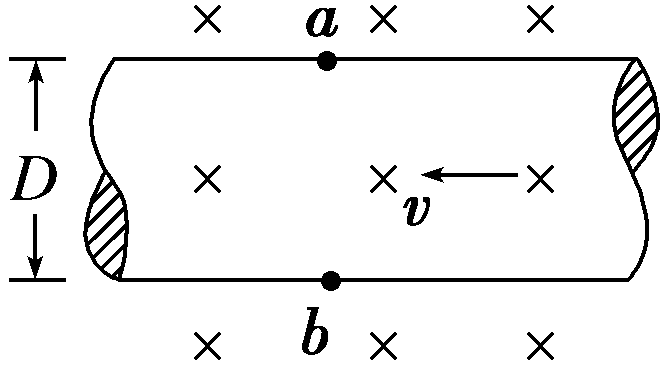
\includegraphics{1.png}
  >>
  所示是图片.其中有四个选项,分别是
  所示是图片.其中有四个选项,分别是
  所示是图片.其中有四个选项,分别是
  所示是图片.其中有四个选项,分别是
  所示是图片.其中有四个选项,分别是
  A.选项A
  B.选项B
  C.选项C
  D.选项D

  a.ABCD

  1.这是选择题的题干,如
  <<
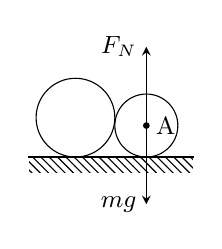
\begin{tikzpicture}
  \draw (-0.5,0.5) circle [radius=0.5]; 
  \draw (0.4,0.4) node [anchor=west] {\small A} circle [radius=0.4];
  \draw [color=white,pattern=north west lines] (-1.1,-0.2)--(-1.1,0)--(1,0)--(1,-0.2);
  \draw (-1.1,0)--(1,0);
  \draw [->,>=stealth] (0.4,0.4) --+(0,-1) node [anchor=east] {\small $mg$};
  \draw [->,>=stealth] (0.4,0.4) --+(0,1) node [anchor=east] {\small $F_N$};
  \filldraw (0.4,0.4) circle [radius=1pt];
\end{tikzpicture}
\qquad
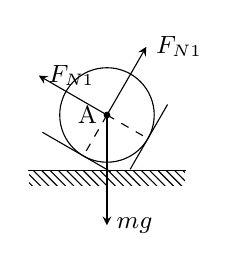
\begin{tikzpicture}
  \draw (0,0.7) node [anchor=east] {\small A} circle [radius=0.6]; 
  \draw [color=white,pattern=north west lines] (-1,-0.2)--(-1,0)--(1,0)--(1,-0.2);
  \draw (-1,0)--(1,0);
  \draw (0,0.7)++(240:0.6)--+(150:0.6);
  \draw (0,0.7)++(240:0.6)--+(330:0.4);
  \draw (0,0.7)++(330:0.6)--+(60:0.5);
  \draw (0,0.7)++(330:0.6)--+(240:0.45);
  \filldraw (0,0.7) circle [radius=1pt];
  \draw [->,>=stealth] (0,0.7)--+(0,-1.4) node [anchor=west] {\small $mg$};
  \draw [->,>=stealth] (0,0.7)--+(150:1) node [anchor=west] {\small $F_{N1}$};
  \draw [->,>=stealth] (0,0.7)--+(60:1) node [anchor=west] {\small $F_{N1}$};
  \draw [dashed](0,0.7)--++(240:0.6);
  \draw [dashed](0,0.7)--++(330:0.6);
\end{tikzpicture}
\qquad
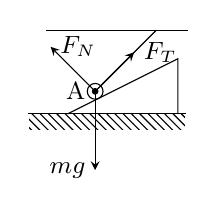
\begin{tikzpicture}
  \draw [color=white,pattern=north west lines] (-1,-0.2)--(-1,0)--(1,0)--(1,-0.2);
  \draw (-1,0)--(1,0);
  \draw (-0.5,0)--(0.9,0.7)--(0.9,0);
  \draw (-0.1,0.2)++(120:0.1) node [anchor=east] {\small A} circle [radius=0.1];
  \draw (-0.1,0.2)++(120:0.1)++(45:0.1)--+(45:1);
  \draw (-0.1,0.2)++(120:0.1)++(45:0.1)++(45:1)--+(0.4,0);
  \draw (-0.1,0.2)++(120:0.1)++(45:0.1)++(45:1)--+(-1.4,0);
  \filldraw (-0.1,0.2)++(120:0.1) circle [radius=1pt];
  \draw [->,>=stealth] (-0.1,0.2)++(120:0.1)--+(0,-1) node [anchor=east] {\small $mg$}; 
  \draw [->,>=stealth] (-0.1,0.2)++(120:0.1)--+(135:0.8) node [anchor=west] {\small $F_N$};
  \draw [->,>=stealth] (-0.1,0.2)++(120:0.1)--+(45:0.7) node [anchor=west] {\small $F_T$};
\end{tikzpicture}
\qquad
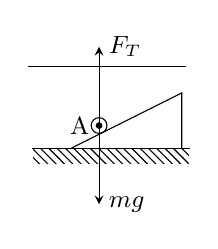
\begin{tikzpicture}
  \draw [color=white,pattern=north west lines] (-1,-0.2)--(-1,0)--(1,0)--(1,-0.2);
  \draw (-1,0)--(1,0);
  \draw (-0.5,0)--(0.9,0.7)--(0.9,0);
  \draw (-0.1,0.2)++(120:0.1) node [anchor=east] {\small A} circle [radius=0.1];
  \draw (-0.1,0.2)++(120:0.1)++(0,0.1)--+(0,0.65);
  \draw (-0.1,0.2)++(120:0.1)++(0,0.1)++(0,0.65)--+(1.1,0);
  \draw (-0.1,0.2)++(120:0.1)++(0,0.1)++(0,0.65)--+(-0.9,0);
  \filldraw (-0.1,0.2)++(120:0.1)  circle [radius=1pt];
  \draw [->,>=stealth] (-0.1,0.2)++(120:0.1) --+(0,-1) node [anchor=west] {\small $mg$};
  \draw [->,>=stealth] (-0.1,0.2)++(120:0.1) --+(0,1) node [anchor=west] {\small $F_T$};
\end{tikzpicture}
  >>
  所示是图片.其中有四个选项,分别是
  所示是图片.其中有四个选项,分别是
  所示是图片.其中有四个选项,分别是
  所示是图片.其中有四个选项,分别是
  所示是图片.其中有四个选项,分别是
  A.选项A选项A选项A选项A选项A选项A选项A选项A选项A选项A选项A
  B.选项B
  C.选项C
  D.选项D

\end{choices}

这是输入选择题后的测试文本缩进的文字.
这是输入选择题后的测试文本缩进的文字.
这是输入选择题后的测试文本缩进的文字.
这是输入选择题后的测试文本缩进的文字.
这是输入选择题后的测试文本缩进的文字.
\newpage
\begin{blanks}
1.这是计算题的题干
这是\blank{计算题}的题干这是计算题的题干
\begin{equation}
  E=MC^2
\end{equation}
这是计算题的题干这是\blank{计算题}的题干
<<
\begin{tikzpicture}
  \draw (0,0) rectangle (3,3);
\end{tikzpicture}
>>
这是计算题的题干这是计算题的题干
这是计算题的题干这是计算题的题干

a.*

1.这是计算题的题干
这是计算题的题干这是计算题的题干
\begin{equation}
  E=MC^2
\end{equation}
这是计算题的题干这是计算题的题干
<<
\begin{tikzpicture}
  \draw (0,0) rectangle (3,2);
\end{tikzpicture}
>>
这是计算题的题干这是计算题的题干
这是计算题的题干这是计算题的题干
这是计算题的题干这是计算题的题干
这是计算题的题干这是计算题的题干
这是计算题的题干这是计算题的题干
这是计算题的题干这是计算题的题干
这是计算题的题干这是计算题的题干
这是计算题的题干这是计算题的题干
这是计算题的题干这是计算题的题干
  
1.这是计算题的题干
这是计算题的题干这是计算题的题干
\begin{equation}
  E=MC^2
\end{equation}
这是计算题的题干这是计算题的题干
<<
\begin{tikzpicture}
  \draw (0,0) rectangle (3,3);
\end{tikzpicture}
>>
这是计算题的题干这是计算题的题干
这是计算题的题干这是计算题的题干

\end{blanks}


\newpage

\begin{judgements}
  1.这是判断题的输出测试,用来排版判断题.

1.这是计算题的题干
这是计算题的题干这是计算题的题干
\begin{equation}
  E=MC^2
\end{equation}
这是计算题的题干这是计算题的题干
<<
\begin{tikzpicture}
  \draw (0,0) rectangle (3,3);
\end{tikzpicture}
>>
这是计算题的题干这是计算题的题干
这是计算题的题干这是计算题的题干

e.这是判断题的解析.2019年9月3日晚完成了全部内容.

\end{judgements}

\begin{calculations}
  1.这是判断题的输出测试,用来排版判断题.

1.这是计算题的题干
这是计算题的题干这是计算题的题干
\begin{equation}
  E=MC^2
\end{equation}
这是计算题的题干这是计算题的题干
<<
\begin{tikzpicture}
  \draw (0,0) rectangle (3,2);
\end{tikzpicture}
>>
这是计算题的题干这是计算题的题干
这是计算题的题干这是计算题的题干
这是计算题的题干这是计算题的题干
这是计算题的题干这是计算题的题干
这是计算题的题干这是计算题的题干
\qitem 第一小问.
\qitem 第二小问.

e.这是判断题的解析.2019年9月3日晚完成了全部内容.

2.各物体受力分析如下
<<
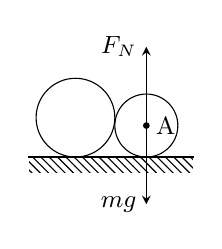
\begin{tikzpicture}
  \draw (-0.5,0.5) circle [radius=0.5]; 
  \draw (0.4,0.4) node [anchor=west] {\small A} circle [radius=0.4];
  \draw [color=white,pattern=north west lines] (-1.1,-0.2)--(-1.1,0)--(1,0)--(1,-0.2);
  \draw (-1.1,0)--(1,0);
  \draw [->,>=stealth] (0.4,0.4) --+(0,-1) node [anchor=east] {\small $mg$};
  \draw [->,>=stealth] (0.4,0.4) --+(0,1) node [anchor=east] {\small $F_N$};
  \filldraw (0.4,0.4) circle [radius=1pt];
\end{tikzpicture}
\qquad
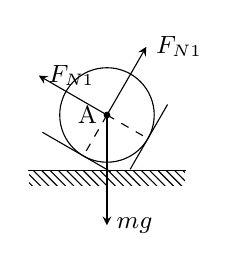
\begin{tikzpicture}
  \draw (0,0.7) node [anchor=east] {\small A} circle [radius=0.6]; 
  \draw [color=white,pattern=north west lines] (-1,-0.2)--(-1,0)--(1,0)--(1,-0.2);
  \draw (-1,0)--(1,0);
  \draw (0,0.7)++(240:0.6)--+(150:0.6);
  \draw (0,0.7)++(240:0.6)--+(330:0.4);
  \draw (0,0.7)++(330:0.6)--+(60:0.5);
  \draw (0,0.7)++(330:0.6)--+(240:0.45);
  \filldraw (0,0.7) circle [radius=1pt];
  \draw [->,>=stealth] (0,0.7)--+(0,-1.4) node [anchor=west] {\small $mg$};
  \draw [->,>=stealth] (0,0.7)--+(150:1) node [anchor=west] {\small $F_{N1}$};
  \draw [->,>=stealth] (0,0.7)--+(60:1) node [anchor=west] {\small $F_{N1}$};
  \draw [dashed](0,0.7)--++(240:0.6);
  \draw [dashed](0,0.7)--++(330:0.6);
\end{tikzpicture}
\qquad
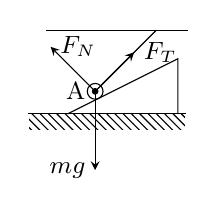
\begin{tikzpicture}
  \draw [color=white,pattern=north west lines] (-1,-0.2)--(-1,0)--(1,0)--(1,-0.2);
  \draw (-1,0)--(1,0);
  \draw (-0.5,0)--(0.9,0.7)--(0.9,0);
  \draw (-0.1,0.2)++(120:0.1) node [anchor=east] {\small A} circle [radius=0.1];
  \draw (-0.1,0.2)++(120:0.1)++(45:0.1)--+(45:1);
  \draw (-0.1,0.2)++(120:0.1)++(45:0.1)++(45:1)--+(0.4,0);
  \draw (-0.1,0.2)++(120:0.1)++(45:0.1)++(45:1)--+(-1.4,0);
  \filldraw (-0.1,0.2)++(120:0.1) circle [radius=1pt];
  \draw [->,>=stealth] (-0.1,0.2)++(120:0.1)--+(0,-1) node [anchor=east] {\small $mg$}; 
  \draw [->,>=stealth] (-0.1,0.2)++(120:0.1)--+(135:0.8) node [anchor=west] {\small $F_N$};
  \draw [->,>=stealth] (-0.1,0.2)++(120:0.1)--+(45:0.7) node [anchor=west] {\small $F_T$};
\end{tikzpicture}
\qquad
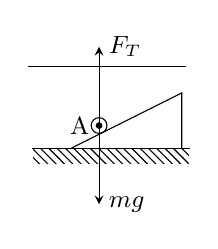
\begin{tikzpicture}
  \draw [color=white,pattern=north west lines] (-1,-0.2)--(-1,0)--(1,0)--(1,-0.2);
  \draw (-1,0)--(1,0);
  \draw (-0.5,0)--(0.9,0.7)--(0.9,0);
  \draw (-0.1,0.2)++(120:0.1) node [anchor=east] {\small A} circle [radius=0.1];
  \draw (-0.1,0.2)++(120:0.1)++(0,0.1)--+(0,0.65);
  \draw (-0.1,0.2)++(120:0.1)++(0,0.1)++(0,0.65)--+(1.1,0);
  \draw (-0.1,0.2)++(120:0.1)++(0,0.1)++(0,0.65)--+(-0.9,0);
  \filldraw (-0.1,0.2)++(120:0.1)  circle [radius=1pt];
  \draw [->,>=stealth] (-0.1,0.2)++(120:0.1) --+(0,-1) node [anchor=west] {\small $mg$};
  \draw [->,>=stealth] (-0.1,0.2)++(120:0.1) --+(0,1) node [anchor=west] {\small $F_T$};
\end{tikzpicture}
>>所示.

\end{calculations}

%\makeanswer

\end{document}
